\chapter{Performance de Programa - Path}

Para realizar a avaliação em questão foram construídas duas configurações do Sistema de Climatização.

\begin{figure}[H]
    \centering
    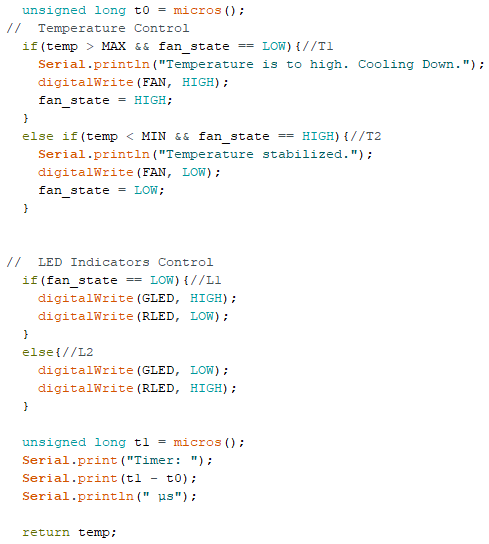
\includegraphics[scale=0.6]{images/path.png}
    \selectlanguage{portuguese}\caption{Melhor Path}
    \label{fig:my_label}
\end{figure}

\begin{table}[H]
    \centering
    \begin{tabular}{|c|c|c|}
        \hline
        \multicolumn{1}{|c|}{Temp.} & 
        \multicolumn{1}{|c|}{Fan} & 
        \multicolumn{1}{|c|}{Path}\\
        \hline
        > MAX & LOW & \makecell{T1 = True \\ L1 = False \& L2 = True}\\
        \hline
        > MAX & HIGH & \makecell{T1 = False \& T2 = False \\ L1 = False \& L2 = True}\\
        \hline
        > MIN \&\& < MAX & LOW & \makecell{T1 = False \& T2 = False \\ L1 = True}\\
        \hline
        > MIN \&\& < MAX & HIGH & \makecell{T1 = False \& T2 = False \\ L1 = False \& L2 = True}\\
        \hline
        < MIN & LOW & \makecell{T1 = False \& T2 = False \\ L1 = True}\\
        \hline
        < MIN & HIGH & \makecell{T1 = False \& T2 = True \\ L1 = True}\\
        \hline
    \end{tabular}
    % \caption{Caption}
    % \label{tab:my_label}
\end{table}

\begin{figure}[H]
    \centering
    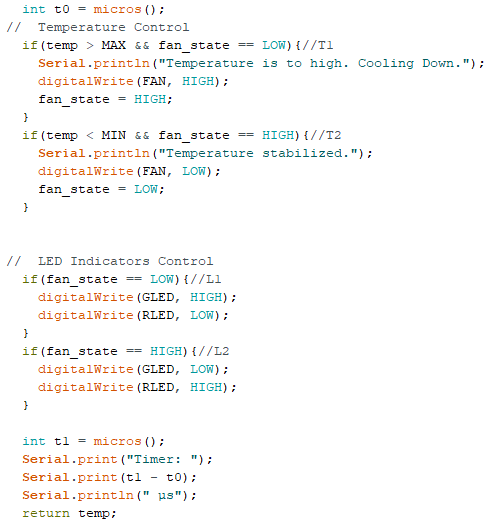
\includegraphics[scale=0.7]{images/path_worst.png}
    \selectlanguage{portuguese}\caption{Pior Path}
    \label{fig:my_label}
\end{figure}

\begin{table}[H]
    \centering
    \begin{tabular}{|c|c|c|}
        \hline
        \multicolumn{1}{|c|}{Temp.} & 
        \multicolumn{1}{|c|}{Fan} & 
        \multicolumn{1}{|c|}{Path}\\
        \hline
        > MAX & LOW & \makecell{T1 = True \& T2 = False\\ L1 = False \& L2 = True}\\
        \hline
        > MAX & HIGH & \makecell{T1 = False \& T2 = False \\ L1 = False \& L2 = True}\\
        \hline
        > MIN \&\& < MAX & LOW & \makecell{T1 = False \& T2 = False \\ L1 = True \& L2 = False}\\
        \hline
        > MIN \&\& < MAX & HIGH & \makecell{T1 = False \& T2 = False \\ L1 = False \& L2 = True}\\
        \hline
        < MIN & LOW & \makecell{T1 = False \& T2 = False \\ L1 = True \& L2 = False}\\
        \hline
        < MIN & HIGH & \makecell{T1 = False \& T2 = True \\ L1 = True \& L2 = False}\\
        \hline
    \end{tabular}
    % \caption{Caption}
    % \label{tab:my_label}
\end{table}

\newpage

\begin{table}[H]
    \centering
    \begin{tabular}{|c|c|c|}
        \hline
        \multicolumn{1}{|c|}{Estado} & \multicolumn{1}{|c|}{Melhor} & \multicolumn{1}{|c|}{Pior}\\ [0.8ex] 
        \hline
        Superior a Máximo               & 280 µs & 300 µs \\
        \hline
        Estável entre Intervalo         & 20 µs & 20 µs \\
        \hline
        Arrefecimento Entre Intervalo   & 20 µs & 20 µs \\
        \hline
        Inferior a Mínimo Arrefecimento & 200 µs & 220 µs \\
        \hline
        Estável Inferior a Mínimo       & 20 µs & 20µs \\
        \hline
    \end{tabular}
    \selectlanguage{portuguese}\caption{Timer}
\end{table}

Apesar de reduzido, é possível verificar uma diferença no desempenho.